% !TeX root = test.tex

%参考文章链接https://dylandong.top/posts/e480/#%E6%AD%A3%E6%96%87

\documentclass[UTF8,12pt,a4paper,oneside]{ctexart}
%指定编码以及文章类型，英文常用：book、article和beamer
%中文常用：ctexbook、ctexart和ctexbeamer

\usepackage{amsmath, amsthm, amssymb, graphicx, bm}
%加载宏包，这里前三个是数学公式，第四个是图片
\usepackage{tabularray}

\title{我的latex笔记}
%文章标题
\author{Nelsonb1}
%作者
\date{\today}
%日期

\newtheorem{theorem}{定理}[section]     %定义定理环境

\usepackage{geometry}                   %设置页边距
\geometry{left=3cm, right=3cm, top=3.8cm, bottom=3cm}
\linespread{1.5}                        %设置行距

%\pagenumbering{roman}                   %设置页码格式，这里设置为罗马数字









%%%%%%%%%%%%%%%%%%%%%%%%%%%%%%%%%%%%%%%%%%%%%%%%%%%%%%%%%%%%%
\begin{document}
%这里面是正文，外面就不是

\maketitle
%在文档中生成标题，不要忘记这个
\newpage
%另起一页
\setcounter{page}{1}
%设置页码，从1开始
\tableofcontents
%生成目录，有目录的文档需要编译两次

\section{一级标题:银临介绍}      %章节

\textbf{Hello 小朋友，中文也支持!}  %加粗，还可设置其他字体

\subsection{二级标题：介绍银临}   %章节

%图片
\begin{figure}[htbp]        %图片，htbp 自动选择最佳位置
	\centering              %图片居中
	
\includegraphics[width=8cm]{银临.jpg}      %插入图片，设置宽度等参数
	\caption{银临本人}                          %图片标题
\end{figure}

%图片
\begin{figure}[htbp]        %图片，htbp 自动选择最佳位置
	\centering              %图片居中
	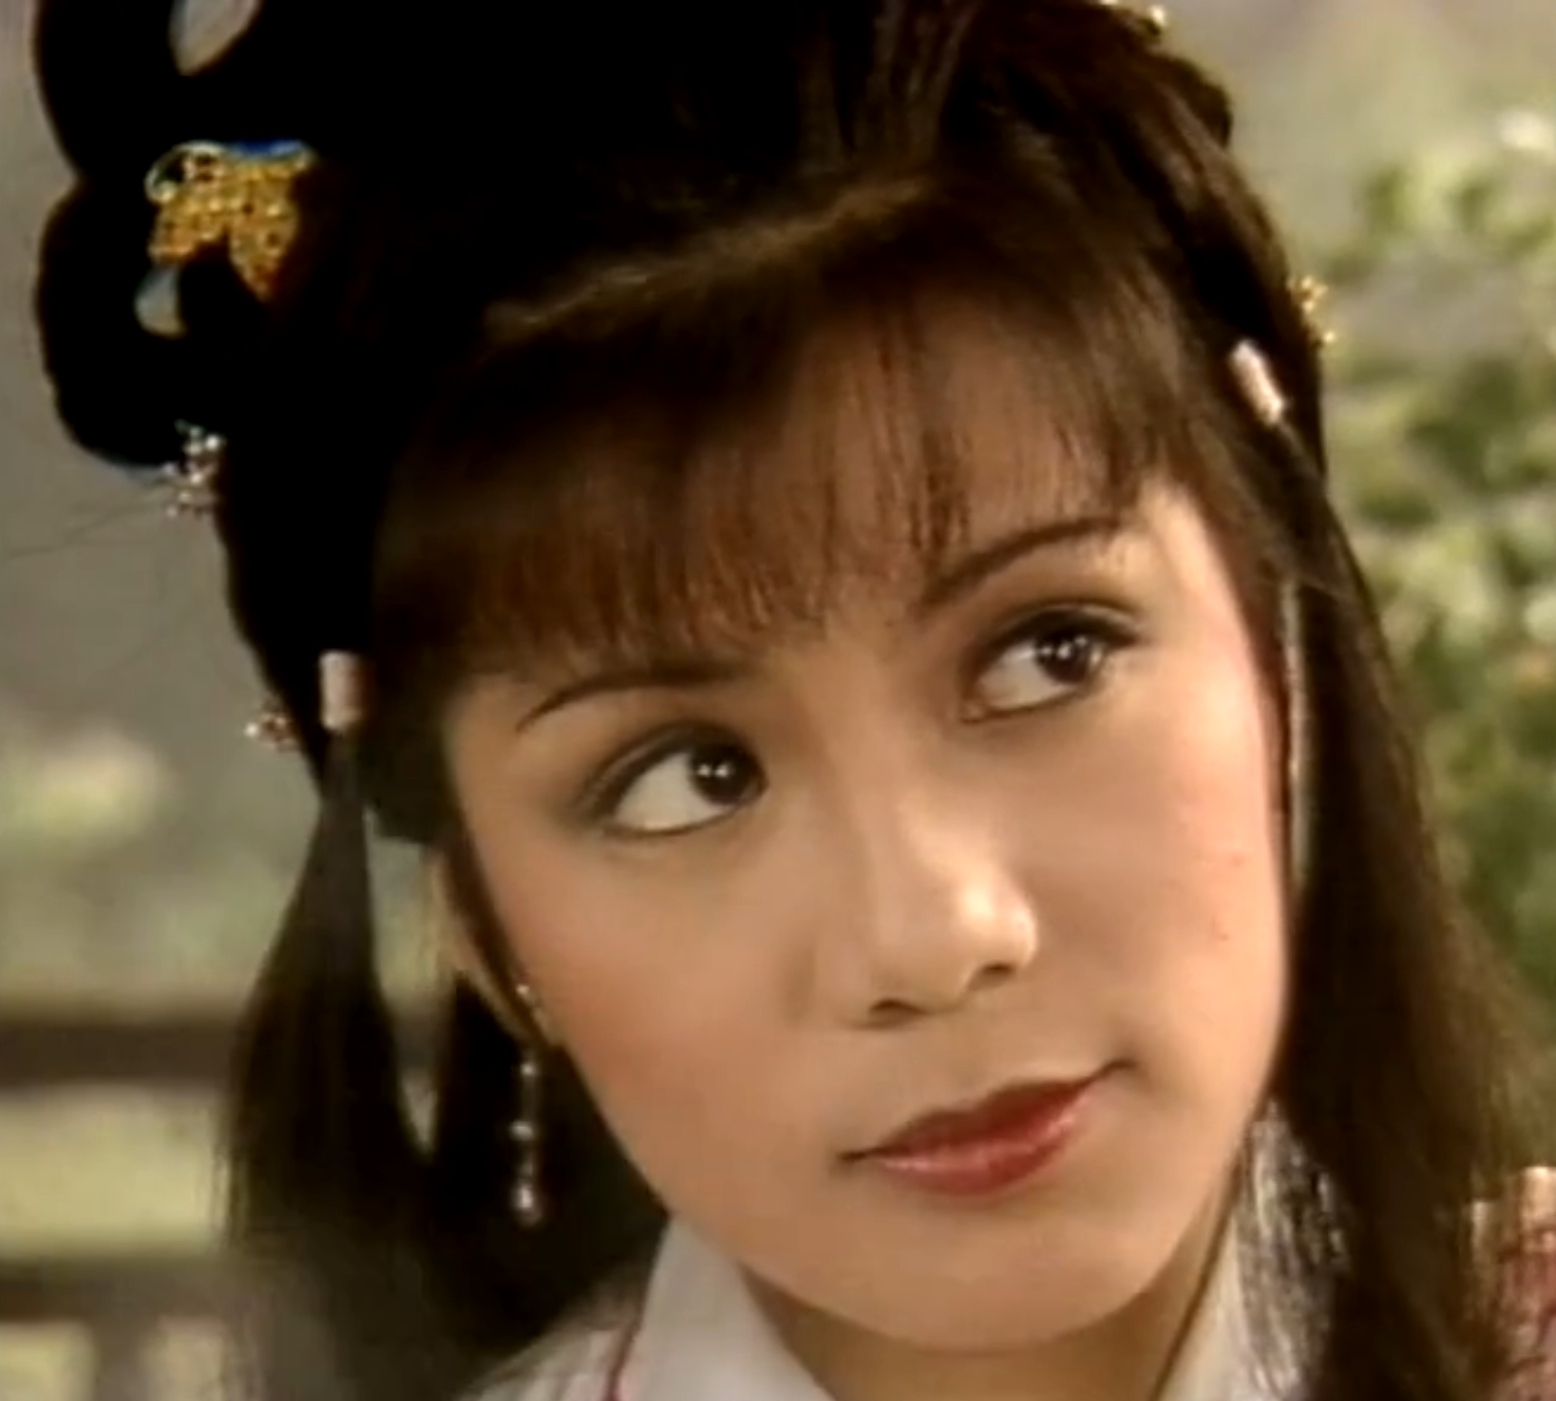
\includegraphics[width=8cm]{黄蓉.png}      %插入图片，设置宽度等参数
	\caption{黄蓉本人}                          %图片标题
\end{figure}

%表格
\begin{table}[htbp]
	\centering
	\caption{代表作品}
	\begin{tabular}{ccc}        %设置表格列数，c为居中，l为左对齐，r为右对齐
        腐草为萤 & 牵丝戏 & 锦鲤抄 \\            %设置表格内容，& 为列分隔符，\\为行分隔符
        不老梦 & 七夕 & 是风动 \\
        7 & 8 & 9
	\end{tabular}
\end{table}

%列表
\begin{enumerate}               %有序列表，还有无序列表itmeize,和描述description
    \item 有序列表;
    \item 裁梦为魂; 
    \item 如一;
    \item 你奔向春野. 
\end{enumerate}

hhhhhhhhhhhhhhhhhhhhhh  

\section{一级标题：许嵩介绍}

%定理环境，需要定义环境，在19行
\begin{theorem}[许嵩三定律]
    \begin{enumerate}
        \item 好歌不一定有人听;
        \item 有人听的不一定是好歌;
        \item 写好歌不需要别人懂.
    \end{enumerate}
\end{theorem}

%证明环境
\begin{proof}
    这是公理，不用证明
\end{proof}

让我们来测试一下行内公式$\frac{BIl}{R}$还行

试下伟大的行间公式
$$
\int_{0}^{\infty} \frac{x^2}{e^x-1} dx = \frac{\pi^2}{12}
$$
逆天好用,试试在线公式编辑https://www.latexlive.com/

\subsection{基本公式写法}
\begin{enumerate}
    \item 上下标：上标\^,下标\_,想括起来用\{\}
    \item 分式：$\dfrac{}{}$,如果想输入较小的分式,用$\frac{}{}$
    \item 括号：直接输\(\),括号内东西高时,用$\left(...\right)$
            $\left(...\middle|...\right)$,中间有分割线,大括号用转义$\{\}$
    \item 加粗：$\bm{}$
    \item 大括号：  用cases环境
                    $$
                    f(x)=\begin{cases}
                        x, & x>0, \\
                        -x, & x\leq 0.
                    \end{cases}
                    $$
    \item 多行公式： 用aligned环境
                    $$
                    \begin{aligned}
                    a & =b+c \\
                    & =d+e
                    \end{aligned}
                    $$
    \item 矩阵、行列式： 矩阵可以用bmatrix环境和pmatrix环境,分别为方括号和圆括号
                    $$
                    \begin{bmatrix}
                        a & b \\
                        c & d
                    \end{bmatrix}
                    $$
\end{enumerate}
Hey there!

\begin{table}[htbp]
    \centering
    \begin{tabular}{llll} 
    \hline
    表头一  & 表头2 & 三                    & 四    \\ 
    \hline
    图片一i &     &                      & 图片四  \\
         &     & \multicolumn{1}{c}{} &      \\
         & 急急急 &                      &      \\
         &     & 滚滚滚                  &      \\
    \hline
    \end{tabular}
    \end{table}
goodbye!
\end{document}